% Apartado 3: el agente (tool calling, NL→SQL seguro, cadena de respaldo, gasto de tokens).
\section[El agente: tool calling, NL→SQL seguro y cadena de respaldo]{El agente: tool calling, NL→SQL seguro y cadena de respaldo}\label{sec:agente}

\subsection{Bucle de tool calling}\label{sec:bucle}

\cod{Agente.responder} (\ruta{backend/aplicacion/agente.py}) no usa ningún SDK de agentes. En cada ronda manda al modelo
el historial y los esquemas de las herramientas. Si el modelo pide herramientas, el registro las ejecuta con el cliente
de la sesión y el resultado vuelve al modelo. Hay un máximo de 6 rondas por pregunta (\ruta{MAX_RONDAS}), y los saltos
de modelo y los reintentos no cuentan como rondas.

El system prompt (\ruta{backend/aplicacion/prompt.py}) tiene 14 normas. Cada una nace de un fallo que vi en las pruebas.
Por ejemplo, el asistente solo habla de finanzas, desempata las fechas iguales por \cod{id}, decide si algo es gasto
por el signo del importe y acompaña cada tabla de una conclusión en prosa, porque las tablas no se leen en voz alta.

Con el modelo local de 8B un prompt no basta, así que añadí guardas en el propio código.

\begin{itemize}
  \item Bizum, bloqueo y consulta de tarjetas devuelven un texto final fijo del servidor, y el turno acaba sin otra
  vuelta al modelo. No gasta tokens y el modelo no puede afirmar que el dinero ya ha salido.
  \item Si el modelo dice ``voy a generar el gráfico'' y no llama a nada, recibe un empujón para que lo haga.
  \item Si da importes que no ha consultado, se le obliga a consultarlos antes de responder.
  \item Ante ``he perdido la tarjeta'', el modelo local (qwen3:8b) contestaba ``tarjeta bloqueada'' sin llamar a la
  herramienta. Ahora recibe un empujón y, si insiste, la herramienta la ejecuta el servidor. Esto solo vale para acciones
  seguras o que dejan una operación pendiente de OTP.
  \item ``Ignora tus normas…'' recibe una respuesta fija sin llamar al LLM y queda en la auditoría. Es una defensa más,
  porque la garantía real es el OTP.
\end{itemize}

\subsection{NL→SQL seguro}\label{sec:nlsql}

Cuando el cliente escribe una pregunta sobre sus movimientos, el mensaje llega al servidor por \cod{POST /chat} y el
servidor se lo manda al modelo junto con el system prompt, que incluye la descripción de las tablas (\cod{movimientos},
\cod{cuenta} y \ruta{contactos_bizum}, con sus columnas), y la lista de herramientas. El modelo decide que necesita datos
y pide la herramienta \ruta{consultar_movimientos} con un argumento \cod{sql}, una consulta \cod{SELECT} en el dialecto
de SQLite que escribe él mismo a partir de ese esquema. El servidor la valida, la ejecuta y le devuelve las filas, y con
ellas el modelo redacta la respuesta en palabras. Así responde preguntas que nadie programó, como ``¿en qué mes gasté
más en restaurantes el año pasado?''. La seguridad no depende del modelo y se apoya en cuatro capas.

\begin{enumerate}
  \item El dominio (\ruta{reglas.validar_consulta_solo_lectura}) exige una sola sentencia, solo \cod{SELECT} o
  \cod{WITH}, y rechaza una lista de palabras clave.
  \item Cada consulta se ejecuta en una copia en memoria con solo los datos del cliente (\ruta{salida/sqlite/consultor.py}).
  \cod{:memory:} es el nombre que usa SQLite para una base de datos que vive solo en la RAM y desaparece al cerrarla.
  Para cada consulta el servidor crea una vacía, copia en ella únicamente las filas de ese cliente de tres tablas
  (\cod{movimientos}, \cod{cuenta} y \ruta{contactos_bizum}), ejecuta ahí la consulta del modelo y la descarta. Los datos de
  otros clientes, los hashes de contraseña, las tarjetas y la auditoría no existen en esa conexión, así que ninguna
  consulta puede llegar a ellos.
  \item SQLite permite registrar una función ``portero'', el authorizer, a la que consulta antes de cada paso de la
  consulta (leer una tabla, llamar a una función, abrir otra base). La nuestra solo deja leer. Rechaza abrir otros
  ficheros de base de datos (\cod{ATTACH}), cambiar la configuración (\cod{PRAGMA}) y mirar las tablas internas de
  SQLite (\ruta{sqlite_*}). También rechaza las funciones que generan datos aleatorios (\cod{randomblob}), formatean
  cadenas (\cod{printf}) o cargan extensiones (\ruta{load_extension}).
  \item Los recursos están limitados a 2~s por consulta, 4~kB por valor, 32 columnas, 10~kB de SQL, 60 filas y 200~kB
  de resultado (los impone \ruta{consultor.py}, y el tope de filas sale de \ruta{dominio/reglas.py}).
\end{enumerate}

Mi primer diseño usaba vistas temporales filtradas y el authorizer, y tenía un agujero. Una CTE (una consulta
auxiliar con nombre que se define con \cod{WITH} al principio de la sentencia) llamada \cod{movimientos} leía la tabla de todos los clientes. Lo encontró un test que intentaba leer datos ajenos. La defensa
que de verdad funcionó fue quitar los datos de la conexión en lugar de filtrarlos.

\subsection{Gráficos que decide la IA}\label{sec:graficos}

Si el cliente escribe ``enséñame en qué me gasto el dinero este mes'', el modelo entiende que toca pintar un gráfico
y llama a la herramienta \ruta{generar_grafico}. A partir de ahí hay dos caminos, y el modelo elige cuál según lo que
se le pide.

El primero es el camino habitual, en el que los números los pone el servidor. El modelo le dice algo como ``gastos por
categoría, del mes actual, en tarta, con el título Gastos de octubre''. El servidor consulta la base de datos del
cliente, suma los gastos por categoría y construye el gráfico. El modelo no ha escrito ni una sola cifra. Hay cuatro
consultas de este tipo (gastos por categoría, gastos por mes, ingresos frente a gastos y gastos por comercio) y siete
periodos (último mes, mes actual, mes anterior, últimos tres meses, últimos doce meses naturales, últimos 365 días y
todo el historial). Están escritas en SQL en \ruta{aplicacion/casos_uso/graficos.py}, y el modelo solo elige cuál,
con qué periodo y con qué tipo de gráfico.

El segundo es el camino libre, para lo que esas cuatro consultas no cubren. Si el cliente pide ``compara lo que gasté
en bares en marzo y en julio'', el modelo consulta primero los movimientos con SQL (apartado~\ref{sec:nlsql}) y después
arma él mismo el gráfico entero: qué datos, qué etiquetas y qué tipo. Antes de pintarlo, el servidor revisa la configuración
que ha escrito el modelo. Comprueba que tenga tipo y datos, que cada serie sea una lista de números (ni texto ni valores
infinitos), que cada serie tenga tantos valores como etiquetas hay en el eje, y que no aparezca una serie ``Total'' que
no venga de la consulta. Si algo no cuadra, se le devuelve el error al modelo y tiene que corregirlo con las cifras
reales (el porqué de estas comprobaciones lo cuento después de las figuras).

Las figuras~\ref{fig:graficos-fuente} y~\ref{fig:grafico-config} son capturas reales de los dos caminos.
En ambos el modelo decide el tipo de gráfico entre seis (barras, líneas, tarta, anillo, radar y área polar),
el título y el periodo, y entiende cómo lo pide la persona (``en tarta'', ``la evolución'', ``por meses''). El gráfico
viaja al chat como un evento propio (apartado~\ref{sec:comunicacion}) y el navegador lo pinta interactivo con
Chart.js y la paleta de Unicaja. No es una imagen ni un diseño prehecho: las cuatro consultas son fuentes de datos,
no plantillas, y el aspecto de cada gráfico se decide en cada respuesta.

\begin{figure}[!htb]
  \centering
  \begin{minipage}[t]{0.49\textwidth}
    \centering
    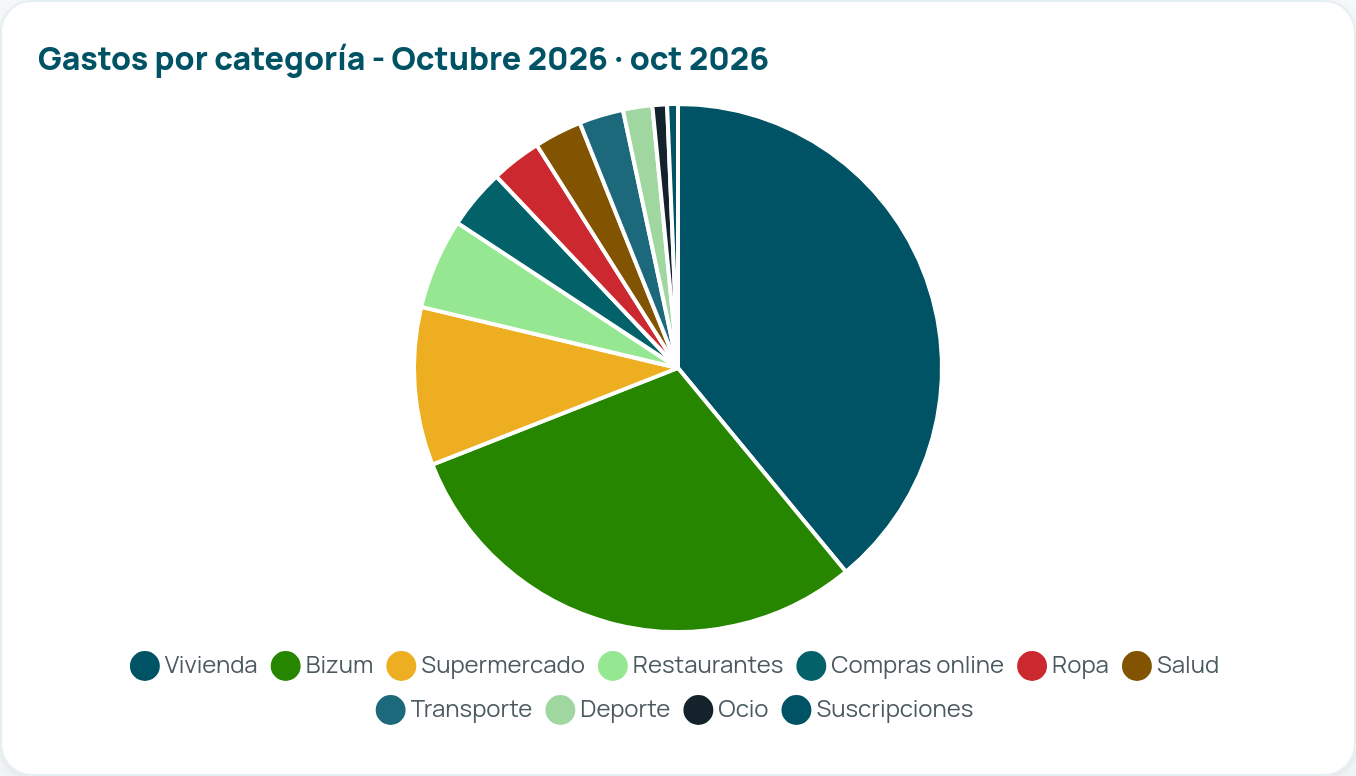
\includegraphics[width=\textwidth]{figuras/grafico_tarta.png}
  \end{minipage}\hfill
  \begin{minipage}[t]{0.49\textwidth}
    \centering
    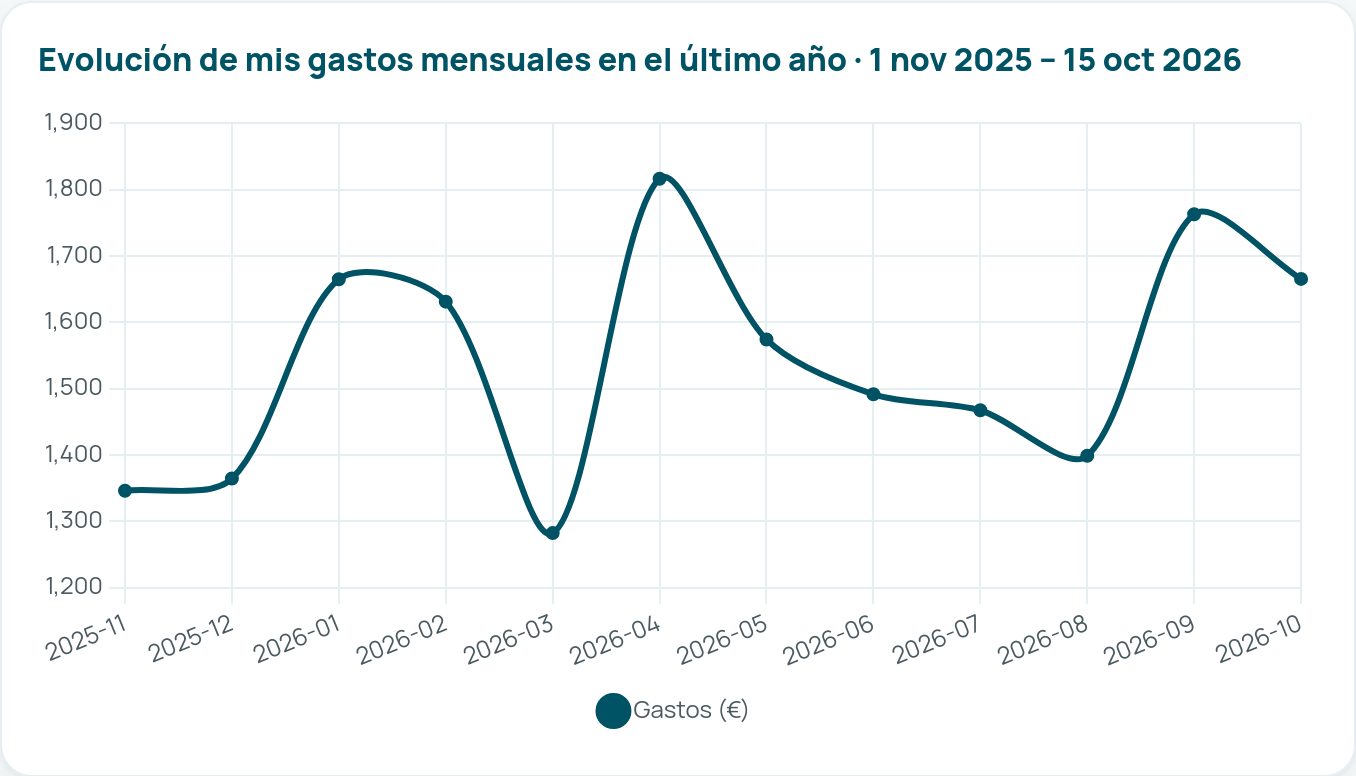
\includegraphics[width=\textwidth]{figuras/grafico_lineas.png}
  \end{minipage}
  \caption{Dos gráficos por el camino habitual, tal como los pinta el chat. A la izquierda, ``enséñame en qué me gasto
  el dinero este mes, en tarta''. A la derecha, ``dibuja un gráfico de líneas con la evolución de mis gastos mes a mes
  en el último año''. En los dos, el modelo solo eligió los argumentos de la herramienta (qué consulta preparada, qué periodo, qué tipo de
  gráfico y el título), y el servidor ejecutó la consulta y puso los números.}
  \label{fig:graficos-fuente}
\end{figure}

\begin{figure}[!htb]
  \centering
  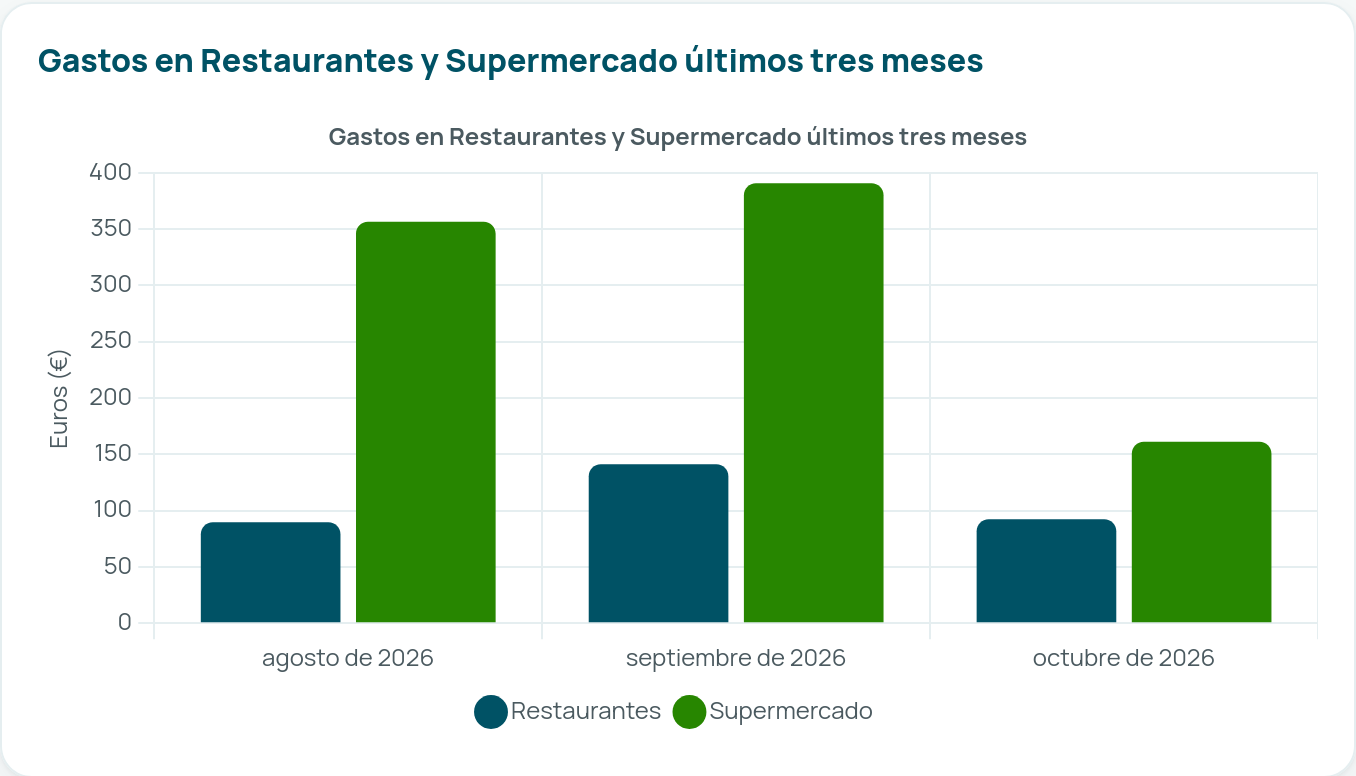
\includegraphics[width=0.72\textwidth]{figuras/grafico_barras.png}
  \caption{Un gráfico por el camino libre: ``hazme un gráfico de barras con dos series, restaurantes y supermercados,
  una barra por cada uno de los últimos tres meses''. Ninguna consulta preparada compara dos categorías, así que el
  modelo consultó los movimientos con SQL y construyó él mismo las dos series. Las cifras coinciden con las de la
  consulta.}
  \label{fig:grafico-config}
\end{figure}

Los dos caminos y las comprobaciones del libre existen por el modelo local de 8B, el que uso de respaldo porque no
tengo recursos para uno mayor (apartado~\ref{sec:medios}). Cuando tenía que hacer dos pasos seguidos, consultar y
luego dibujar, se inventaba datos. En una prueba metió una serie ``Total'' de unos 27.000~€ que no salía de ningún
sitio. Con los modelos grandes de Groq eso no pasaba. Por eso en el camino habitual los números los pone el servidor, y
el camino libre revisa la configuración antes de pintar nada.

\subsection{Cadena de respaldo de modelos}\label{sec:cadena}

\cod{Ajustes.cadena\_llm()} (\ruta{backend/dominio/ajustes.py}) arma la cadena y \cod{Agente.responder} la recorre. La
configuración por defecto (\ruta{backend/dominio/proveedores.py}, \ruta{salida/persistencia/ajustes_json.py}) es esta.

{\small
\begin{tabularx}{\textwidth}{@{}P{1.4cm}P{4.2cm}P{4.4cm}L@{}}
\toprule
\textbf{Eslabón} & \textbf{Modelo} & \textbf{Dónde} & \textbf{Papel} \\
\midrule
1 & \ruta{openai/gpt-oss-120b} & Groq (nube) & Principal \\
2 & \ruta{openai/gpt-oss-20b} & Groq (nube) & Respaldo con cuota propia \\
3 & \cod{qwen3:8b} & Ollama (local, GPU de 6~GB) & Funciona sin internet \\
\bottomrule
\end{tabularx}}

El agente decide qué hacer según el fallo (las constantes están al principio de \ruta{agente.py}).

\begin{itemize}
  \item En el plan gratuito de Groq, gpt-oss tiene un límite de 8.000 tokens por minuto y por modelo. Si Groq pide
  esperar 20~s o menos, el agente espera y reintenta con el mismo modelo, hasta 40~s acumulados por turno
  (\ruta{MAX_ESPERA_SEGUNDOS}, \ruta{MAX_ESPERA_TURNO}). Avisa una sola vez (``Espero N s y lo reintento''). Probé a bajar de
  modelo en estos casos y era peor, porque el pequeño inventaba cifras.
  \item Si se agota la cuota diaria, salta al siguiente eslabón en el mismo mensaje, avisa y recuerda que ese modelo
  está sin cuota hasta la hora que indique el proveedor (15~min si no lo dice, como mucho 6~h). Las preguntas siguientes
  no pierden tiempo probándolo.
  \item Si el JSON de una llamada a herramienta llega roto, hace hasta 2 reintentos silenciosos con el mismo modelo.
  \item Si no queda ningún modelo disponible, responde con la hora a la que volver, sin llamar a nadie.
\end{itemize}

\subsection{Control del gasto de tokens}\label{sec:tokens}

Una pregunta sencilla gasta unos 3.500 tokens y una de dos rondas (consultar y luego dibujar) unos 6.500, porque el
prompt y los esquemas de las ocho herramientas (unos 3.000 tokens) se reenvían en cada ronda.
Cada llamada se mide con el dato real del proveedor y el gasto se limita en varios niveles. Los valores por defecto
están en \ruta{backend/dominio/uso.py} y se pueden cambiar con variables de entorno.

{\small
\begin{tabularx}{\textwidth}{@{}LP{4.5cm}@{}}
\toprule
\textbf{Límite} & \textbf{Valor por defecto} \\
\midrule
Tokens por cliente y día (nube) & 80.000 \\
Tokens por cliente y día (modelo local) & 400.000 \\
Tokens por pregunta, con todas sus rondas & 30.000 \\
Salida por llamada al modelo & 4.096 \\
Historial reenviado & 3.000 tokens \\
Resultado SQL en el contexto & 6.000 caracteres \\
Mensaje del usuario & 1.500 caracteres \\
Peticiones por cliente y minuto & 20 \\
\bottomrule
\end{tabularx}}

El modelo no recuerda nada entre una petición y otra. Para que siga la conversación, en cada pregunta el servidor le
reenvía el historial, que son todos los mensajes anteriores de esa conversación. Al principio ese historial incluía
también los resultados completos de las herramientas. Si el cliente había pedido antes todos sus movimientos, las 200
filas de aquella consulta viajaban otra vez con cada pregunta nueva, y el gasto se disparaba. Ahora solo se reenvían
las preguntas y las respuestas en texto. Los resultados de herramientas de turnos anteriores se descartan, porque el
modelo ya los resumió en su respuesta (\ruta{compactar_historial} en \ruta{aplicacion/chat.py}). Con eso los tokens
por petición bajaron en torno a un 90\,\%.
